\chapter{Σχεδιασμός και υλοποίηση}
\label{chap:implementation}

Όπως είδαμε στο προηγούμενο κεφάλαιο κανένα unikernel framework δεν υποστηρίζει
την κλήση συστήματος fork και επομένως εφαρμογές που χρησιμοποιούν τη
συγκεκριμένη κλήση δεν μπορούν να υποστηριχτούν από αυτά. Στο πλαίσιο, λοιπόν,
της παρούσας διπλωματικής εργασίας δημιουργήσαμε ένα μηχανισμό που
υλοποιεί τις κλήσεις συστήματος fork και pipe σε KVM hypervisor. Ο στόχος ήταν
να διατηρηθεί το single proccess χαρακτηριστικό των unikernels. Για το λόγο
αυτό το αποτέλεσμα της κλησης fork, δεν είναι η δημιουργία μία νέας διεργασίας
στο υπάρχον unikernel, αλλά η εκκίνηση ενός unikernel, ίδιου με το αρχικό. 

Επιπλέον, υλοποιήθηκε και ένας inter-vm communication μηχανισμός, στα πρότυπα
της κλήσης συστήματος pipe. Δηλαδή δύο εικονικά μηχανήματα μπορούν να
επικοινωνούν μεταξύ τους, όπως δύο διεργασίες επικοινωνούν μεταξύ τους, μέσω της
κλήσης συστήματος pipe, σε ένα λειτουργικό σύστημα γενικού σκοπού. 

Στο παρών κεφάλαιο περιγράφουμε αναλυτικά τους δύο αυτούς μηχανισμούς. Το
κεφάλαιο χωρίζεται σε δύο μέρη, ένα για το μηχανισμό pipe και ένα για το
μηχανισμό fork. Σε κάθε μέρος περιγράφεται αναλυτικά τόσο ο μηχανισμός, όσο και
η διαδικασία και τα στάδια μέχρι την τελική υλοποίηση τους.

\newpage
\section{Μηχανισμός pipe}

Σύμφωνα με το POSIX ο ορισμός της κλήσης συστήματος pipe έχει ως εξής:
\begin{lstlisting}[numbers=none,  xleftmargin=.2\textwidth, xrightmargin=.2\textwidth]
int pipe(int fildes[2]);
\end{lstlisting}
Ο μηχανισμός pipe που υλοποιήθηκε που υλοποιήθηκε ακολουθεί τον ορισμό του
POSIX. Πιο συγκεκριμένα μία κλήση στη συγκεκριμένη συνάρτηση δημιουργεί ένα pipe
μεταξύ των δύο εικονικών μηχανημάτων και δημιουργεί δύο νέους file descriptors.
Οι δύο αυτοι file descriptors αποθηκεύονται στις παραμέτρους fildes[0] και
fildes[1]. Ο πρώτος file descriptor αφορά το read κομμάτι του pipe, ενώ ο
δεύτερος το write κομμάτι του pipe. Η τιμή που επιστρέφει η κλήση συστήματος
είναι 0, αν η δημιουργία του pipe ήταν επιτυχής, ενώ διαφορετικά θα επιστραφεί
-1 και η μεταβλητή errno περιέχει την τιμή του σφάλματος.

Η ανάγνωση από το pipe γίνεται χρησιμοποιώντας τον πρώτο file descriptor από τις
παραμέτρους της κλήσης. Τα δεδομένα διαβάζονται με FIFO (first in first out)
σειρά. Ενώ αν δεν υπάρχουν δεδομένα στο pipe τότε η κλήση "μπλοκάρει" μέχρι να
προκύψουν δεδομένα από το write άκρο του pipe. Η εγγραφή στο pipe γίνεται
χρησιμοποιώντας το δεύτερο file descriptor από τις παραμέτρους της κλήσης. Η
εγγραφή στο pipe μπορεί να μπλοκάρει αν δεν υπάρχει χώρος στο pipe. Επιπλέον
μπορεί να αποτύχει αν όλα τα file descriptos για ανάγνωση από το pipe έχουν
κλείσει με το σφάλμα EPIPE. 

\subsection{Στάδια υλοποίησης}

Η υλοποίηση του συγκεκριμένου μηχανσιμού έγινε σε 3 στάδια, τα οποία αναλύονται
παρακάτω. 

\subsubsection{Στάδιο 1 - επίπεδο εφαρμογής}

%%Στο πρώτο στάδιο, δημιουργήσαμε μία επικοινωνία μεταξύ των unikernels,
%%χρησιμοποιώντας TCP/IP sockets. Όπως φαίνεται στην παρακάτω εικόνα \ref{fig4_1}
%%όλη η εργασία για τη δημιουργία της επικοινωνίας γινόταν μέσα από την  εφαρμγοή
%%που εκτελούνταν στο unikernel. Δεδομένου της χρήσης των sockets, κάποιο
%%unikernel θα έπρεπε να είχε το ρόλο του server και το άλλο το ρόλο του client.
%%Όπως γίνεται εύκολα κατανοητό, ο συγκεκριμένος μηχανισμός απαιτεί την ύπαρξη
%%σύνδεσης σε κάποιο κοινό δίκτυο για τα δύο εικονικα μηχανήματα.

Στο πρώτο στάδιο, υλοποιήσαμε το pipe ως μία συνάρτηση που καλείται από την
εφαμρογή. Η συνάρτηση αυτή χρησιμοποιεί TCP/IP sockets για να εγκαθιδρύσει την
επικοινωνία μεταξύ ρων δύο εφαρμογών. Συγκεκριμένα χρησιμοποιούνται δύο sockets,
ένα για την αποστολή δεδομένων και ένα για την παραλαβή. Οι file descriptors των
των δύο αυτών sockets, είναι και οι τιμές που αποθηκεύονται στις μεταβλητές
fildes[0] και fildes[1]. Στην παρακάτω εικόνα \ref{fig4_1} φαίνεται σχηματικά η
υλοποίηση.

\begin{figure}[htp]
\centering
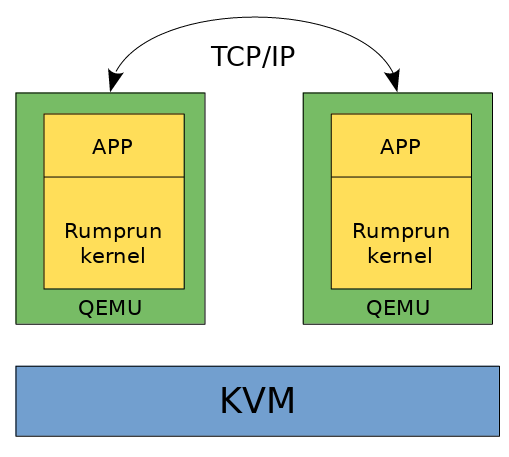
\includegraphics[scale=0.7]{figures/pipe_stage1_function.png}
\caption{Πρώτο στάδιο υλοποίησης μηχανισμού pipe\label{fig4_1}}
\end{figure}

Όπως γίνεται εύκολα κατανοητό η συγκεκριμένη υλοποίηση απαιτεί την ύπαρξη
δικτύου ανάμεσα στα δύο εικονικά μηχανήματα. Επιπλέον, λόγω της χρήσης των
sockets, δεν υλοποιήθηκε όλα τα semantics του pipe. Έτσι ακόμα και αν δεν
υπάρχει ανοιχτό read άκρο στο pipe, οποιαδήποτε εγγραφή στο pipe θα είναι
επιτυχής. Ακόμα, οποιαδήποτε εγγραφή μπορεί να μπλοκάρει μόνο αν ο παραλήπτης
δεν μπορεί να δεχτεί άλλα δεδομένα. Αντιθέτως τα semantics του άκρου ανάγνωσης
του pipe διατηρήθηκαν καθώς και στην περίπτωση των sockets, αν δεν υπάρχουν
δεδομένα προς ανάγνωση η αντίστοιχη κλήση "μπλοκάρει". 

Για να υλοποιηθεί η συνάρτηση pipe, ακολουθήθηκε η ίδια διαδικασία που
ακολουθείται από μία εφαρμογή για να επικοινωνήσει με κάποια άλλη μέσω δικτύου.
Η διαφορά είναι ότι η εφαρμογή έχει το ρόλο του server και του client
ταυτόχρονα. Για αυτό το λόγο χρησιμοποιήθηκαν δύο sockets, ένα για κάθε ρόλο. 
Στην παρακάτω εικόνα \ref{fig4_2} φαίνεται η αλληλουχία κλήσεων συστήματος για
την εγκαθίδρυση της επικοινωνίας (server/client). 

%%O συγκεκριμένος μηχανισμός επικοινωνίας είναι ακριβώς ίδιος με αυτό που
%%χρησιμοποιούν δύο εφαρμογές για να επικοινωνήσουν μεταξύ τους. Ο τρόπος με τον
%%οποίο δημιουργείται ο μηχανισμός με τις ανάλογες κλήσεις συστήματος φαίνεται
%%στην εικόνα \ref{fig4_2}. Όπως φαίνεται από τη μεριά του o client χρειάζεται να
%%ανοίξει ένα socket, να συνδεθεί με το server χρησιμοποιώντας την connect(). Από
%%τη δικιά του μεριά ο server, μετά τη δημιουργία του socket το δεσμεύει σε μία
%%συγκεκριμένη θύρα χρησιμοποιώντας την bind, θέτει το συγκεκριμένο socket ως
%%passive socket ώστε να δεχτεί νέες συνδέσεις με τη listen() και περιμένει κάποια
%%νέα σύνδεση μπλοκάροντας στην accept(). Το συγκεκριμένο στάδιο αποσκοπούσε
%%κυρίως στην περαιτέρω εξοικείωση με το rumprun unikernel framework. Στη συνέχεια
%%η ενδοεπικοινωνία γινόταν γράφοντας και διαβάζοντας στα file descriptors που
%%είχαν δημιουργηθεί από την παραπάνω διαδικασία. 

\begin{figure}[htp]
\centering
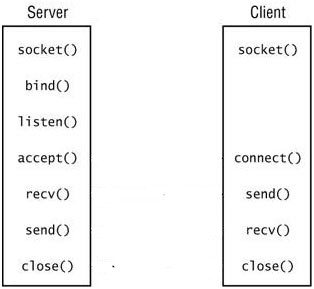
\includegraphics[scale=0.7]{figures/Server_client_syscalls_tcp_ip_socket.jpg}
\caption{Αλληλουχία κλήσεων για επικοινωνία μέσω TCP/IP sockets \label{fig4_2}}
\end{figure}

Η συνάρτηση pipe, λοιπόν ακολουθεί και τις δύο διαδικασίες που φαίνονται
(server/client). Αυτό όμως προξενεί ένα πρόβλημα κατά τη δημιουργία της
επικοινωνίας. Αν και οι δύο εφαρμογές ακολουθήσουν την παραπάνω ακολουθία
κλήσεων τότε θα δημιουργηθεί αδιέξοδο, καθώς και οι 2 θα έχουν κολλήσει στην
κλήση accept, περιμένοντας κάποια σύνδεση. Ο τρόπος με τον οποίο επιλύθηκε το
παραπάνω πρόβλημα είναι ως εξής. Μία από τις δύο εφαρμογές να εκτελεί πρώτα τις
κλήσεις που αφορούν το client κομμάτι και μετά αυτές που αφορούν το server.
Αντίθετα η άλλη εφαρμογή, πρώτα εκτελεί τις κλήσεις που αφορούν το server και
ύστερα αυτές που αφορούν το client μερος. 

\subsubsection{Στάδιο 2 - pipe ως system call με UDP sockets}

Στο δεύτερο στάδιο, υλοποιήσαμε το μηχανισμό του pipe μέσα στον πυρήνα του
rumprun. Ουσιαστικά μετατρέψαμε το function call του προηγούμενου σταδίου σε
system call. Σε αντίθεση με πριν, η επικοινωνία γίνεται μέσω UDP sockets, οπότε
και είναι απαραίτητη η ύπαρξη δικτύου. Η επιλογή του πρωτοκόλλου UDP έναντι του
TCP, έγινε για την πιο εύκολη δημιουργία και χρήση sockets στον πυρήνα του
rumprun. Ο συγκεκριμένος μηχανισμός δίνει τη δυνατότητα να υπάρχει επικοινωνία
μεταξύ δύο ξεχωριστών unikernels, ακόμα και αν αυτά δε μοιράζονται τον ίδιο
host, μέσω μίας κλήσης συστήματος παρόμοια με την pipe(). Με αυτό τον τρόπο, οι
εφαρμογές δε χρειάζονται να τροποποιηθούν σε μεγάλο βαθμό, από την αρχική τους
έκδοση. Στην παρακάτω εικόνα ~\ref{fig4_3} φαίνεται σχηματικά η υλοποίηση.

\begin{figure}[htp]
\centering
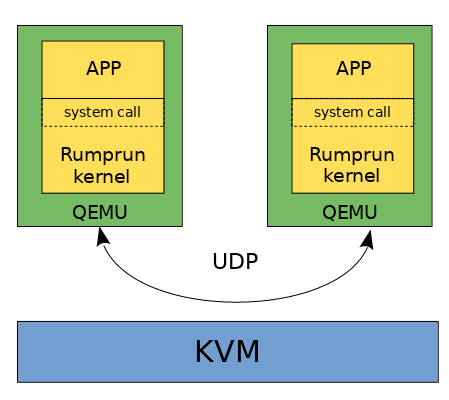
\includegraphics[scale=0.7]{figures/pipe_stage2.png}
\caption{Δεύτερο στάδιο υλοποίησης μηχανισμού pipe\label{fig4_3}}
\end{figure}

Όσον αφορά τη χρήση του μηχανισμού, αυτή γίνεται ακολουθώντας την ίδια
διαδικασία με τη χρήση της κλήσης pipe σε ένα UNIX σύστημα. Στις παραμέτρους
fildes[0], fildes[1], αποθηκεύονται οι δύο file descriptors που θα
χρησιμοποιηθούν για την ανάγνωση και εγγραφή αντίστοιχα. Σε περίπτωση επιτυχίας
επιστρέφεται η τιμή 0, ενώ σε αντίθετη περίπτωση, στη μεταβλητή errno
αποθηκεύεται ο κωδικός του σφάλματος. Δεδομένου, ότι η επικοινωνία γίνεται με
UDP sockets, τα semantics είναι ίδια με το προηγούμενο στάδιο. Μία σημαντική
διαφορά, είναι ότι πρέπει να καθοριστεί η διεύθυνση IP του unikernel με το οποίο
θα εγκαθιδρυθεί η επικοινωνία. Για το λόγο αυτό, μετά την κλήση της pipe() θα
πρέπει μέσω της ioctl στο file descriptor της εγγραφής 
\begin{lstlisting}[numbers=none,  xleftmargin=.05\textwidth, xrightmargin=.05\textwidth]
ioctl(fildes[1], SETIPADDR, htonl(IP_ADDRESS));
\end{lstlisting}
Η μορφή της IP διεύθυνσης θα πρέπει να είναι σε network byte order
και για αυτό το σκοπό μπορεί να χρησιμοποιηθεί η συνάρτηση htonl.
Ο τρόπος που λειτουργεί ο μηχανισμός έχει ως εξής:
\begin{enumerate}
	\item Αρχικά καλώντας την pipe, επιστρέφονται τα δύο απαραίτητα file
		descriptors, ένα για εγγραφή και ένα για ανάγνωση.
	\item Στη συνέχεια, πρεπει να οριστεί η διεύθυνση IP, στην οποία θέλουμε
		να στείλουμε τα δεδομένα. Αυτό γίνεται μέσω της προαναφερθείσας
		ioctl κλήσης. 
	\item Η εφαρμογή στέλνει δεδομένα χρησιμοποιώντας την κλήση write() και
		το file descriptor που αντιπροσωπεύει το άκρο εγγραφής του pipe.
	\item H εφαρμογή λαμβάνει δεδομένα χρησιμοποιώντας την κλήση read() και
		το file descriptor που αντιπροσωπεύει το άκρο ανάγνωσης του pipe.
\end{enumerate}

Η μεταφορά του μηχανισμού στον πυρήνα του rumprun απαιτούσε και τις ανάλογες
αλλαγές στις συναρτήσεις που χρησιμοποιήθηκαν, καθώς πλέον ο προγραμματισμός
γινόταν εντός του πυρήνα. Ο πυρήνας που χρησιμοποιεί το rumprun είναι αυτός του
NetBSD και σε σχέση με τον τρόπο που χρησιμοποιούνται τα sockets σε userspace,
διαφέρει με τον αντίστοιχο σε kernelspace. Ο συγκεκριμένος μηχανισμός
χρησιμοποιεί ένα struct, στο οποίο αποθηκεύονται το socket, το file descriptor
και η διεύθυνση IP του παραλήπτη. 
\begin{lstlisting}[numbers=none,  xleftmargin=.2\textwidth, xrightmargin=.2\textwidth]
struct pipe_data {
	struct socket *so;
	uint32_t ip;
	int fd;
};
\end{lstlisting}
Παρακάτω, περιγράφεται τι γίνεται μέσα στον πυρήνα όταν εκτελούνται οι παραπάνω
κλήσεις. 
\begin{enumerate}
	\item pipe: Αρχικά, δημιουργούνται δύο sockets με την socreate, ένα για
		αποστολή και ένα για παραλαβή δεδομένων και αποθηκεύονται στα
		αντίστοιχα πεδία του struct pipe\_data. Το socket που θα
		χρησιμοποιηθεί για ανάγνωση γίνεται bind στη θύρα 23456 με την
		sobind,	επιτρέποντας συνδέσεις από κάθε IP. Στη συνέχεια,
		δημιουργούνται τα 2 file descriptors που θα χρησιμοποιούνται από
		την εφαρμογή. Τα file descriptos, από τη μεριά του πυρήνα
		αντιπροσωπεύονται από τις δομές file\_t. Στις δομές
		αυτές αποθηκεύεται και το struct pipe\_data που αναφέρθηκε
		προηγουμένως. Αν όλα έχουν πάει καλά, προστίθονται τα δύο file
		descriptors στην εφαρμογή και επιστρέφει με επιτυχία η pipe.
	\item ioctl: Όταν καλείται η ioctl με το command SETIPADDR, αποθηκεύεται
		στο πεδίο ip του pipe\_data η τιμή που έχει περαστεί ως τρίτη
		παράμετρος στην ioctl.
	\item write: Αρχικά αρχικοποιείται το struct sockaddr\_in, το οποίο
		λαμβάνει την IP του παραλήπτη από το πεδίο ip του pipe\_data.
		Στη συνέχεια χρησιμοποιώντας τη sosend, στέλνονται τα δεδομένα
		μέσα από το socket.
	\item read: Με τη χρήση της soreceive, διαβάζονται τυχόν δεδομένα στο
		socket. Αν δεν υπάρχουν δεδομένα η soreceive μπλοκάρει μέχρι να
		προκύψουν.
\end{enumerate}

Στον πυρήνα του NetBSD, τυχόν δεδομένα που μεταφέρονται από userspace σε
kernelspace αποθηκεύονται στο struct uio. Τόσο η soreceive, όσο και η sosend,
δίνουν τη δυνατότητα να χρησιμοποιηθεί το συγκεκριμένο struct και συνεπώς δεν
υπάρχει ανάγκη για παραπάνω αντιγραφές των δεδομένων. Η διαδικασία για την
εισαγωγή μία νέας κλήσης συστήματος στο rumprun, είναι ακριβώς ίδια με αυτή που
θα χρησιμοποιηθεί για την εισαγωγή μία κλήσης συστήματος στον πυρήνα του NetBSD,
με ένα επιπλέον βήμα. Αφού εισαχθεί η κλήση συστήματος στο NetBSD, πρέπει να
εισαχθεί στο αρχείο src-netbsd/sys/rump/librump/rumpkern η κλήση συστήματος.
Σε αυτό το σημείο, καλό είναι να ξανααναφερθεί ότι στα unikernels δεν υπάρχει
διαχωρισμός μεταξύ userspace και kernelspace, ωστόσο οι συγκεκριμένοι όροι
χρησιμοποιούνται για να γίνει διαχωρισμός μεταξύ του κώδικα μίας οποιασδήποτε
εφαρμογής και του κώδικα του πυρήνα του unikernel.

%% -----------------------------------------------------------------------------
%% ------------------------ Deutero stadio me device ---------------------------
%% -----------------------------------------------------------------------------

%%Στο δεύτερο στάδιο, υλοποιήσαμε το μηχανισμό, μέσα στον πυρήνα του rumprun. Όπως
%%και στο προηγούμενο στάδιο, έτσι και εδώ η επικοινωνία γίνεται μέσψ TCP/IP
%%sockets, συνεπώς είναι απαραίτητη η ύπαρξη δικτύου. Βέβαια ο συγκεκριμένος
%%μηχανισμός μπορεί να χρησιμοποιηθεί για την επικοινωνία rumprun unikernels που
%%δε βρίσκονται στον ίδιο host. Ο τρόπος με τον οποίο επιλέχθηκε να γίνει αυτό
%%είναι μέσω μίας ψευδοσυσκευής. Στην παρακάτω εικόνα \ref{fig4_3} φαίνεται 
%%σχηματικά η υλοποίηση.  
%%
%%\begin{figure}[htp]
%%\centering
%%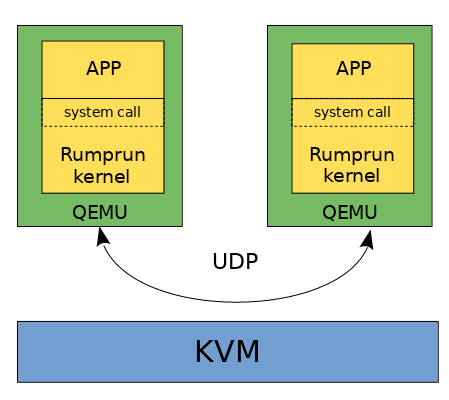
\includegraphics[scale=0.7]{figures/pipe_stage2.png}
%%\caption{Δεύτερο στάδιο υλοποίησης μηχανισμού pipe\label{fig4_3}}
%%\end{figure}
%%
%%Στο επίπεδο της εφαρμογής, ο μηχανισμός είναι διαθέσιμος μέσω της συσκευής
%%/dev/comso. Ανοίγωντας τη συγκεκριμένη συσκευή, η εφαρμογή έχει τη δυνατότητα να
%%στέλνει και να λαμβάνει δεδομένα, γράφοντας και διαβάζοντας αντίστοιχα στη
%%συγκεκριμένη συσκευή. Ουσιαστικά το pipe έχει μετατραπεί σε μία ψευδοσυσκευή που
%%μπορεί να επικοινωνήσει μέσω TCP/IP sockets, με άλλες εφαρμογές. Ο τρόπος με τον
%%οποίο υλοποιήθηκε ο μηχανισμός, αλλάζει τον ορισμό του pipe, καθώς μέσω του
%%ίδιου file descriptor, η εφαρμογή μπορεί να γράψει ή να διαβάσει δεδομένα. Τέλος
%%τα semantics είναι ίδια με το προηγούμενο στάδιο. 
%%
%%Η μεταφορά του μηχανισμού στον πυρήνα του rumprun απαιτούσε και τις ανάλογες
%%αλλαγές στις συναρτήσεις που χρησιμοποιήθηκαν, καθώς πλέον ο προγραμματισμός
%%γινόταν εντός του πυρήνα. Ο πυρήνας που χρησιμοποιεί το rumprun είναι αυτός του
%%NetBSD και σε σχέση με τον τρόπο  που χρησιμοποιούνται τα sockets σε userspace,
%%διαφέρει με τον αντίστοιχο σε kernelspace. Ο τρόπος που λειτουργεί ο μηχανισμός
%%φαίνεται στην εικόνα \ref{fig4_4} και μία σύντομη περιγραφή του έχει ως εξής:
%%\begin{enumerate}
%%	\item Αρχικά η εφαρμογή χεησιμοποιεί την open για να ανοίξει τη συσκευή.
%%		Από τη μεριά του πυρήνα, αυτό έχει ως αποτέλεσμα τη δημιουργία
%%		του socket που θα χρησιμοποιηθεί για την επικοινωνία. Η
%%		δημιουργία του socket γίνεται χρησιμοποιώντας τη sosocket().
%%	\item Η εφαρμογή στέλνει δεδομένα χρησιμοποιώντας την κλήση write() και
%%		το file descriptor που αντιπροσωπεύει την ανοιχτή συσκευή comso.
%%		Από τη μεριά του πυρήνα, όταν λαμβάνεται το συγκεκριμένο αίτημα
%%		χρησιμοπποιείται η sosend, για να σταλούν τα δεδομένα μέσω του
%%		socket στον προορισμό.
%%	\item H εφαμρογή λαμβάνει δεδομένα χρησιμοποιώντας την κλήση open() και
%%		το file descriptor που αντιπροσωπεύει την ανοιχτή συσκευή comso.
%%		Από τη μεριά του πυρήνα, όταν λαμβάνεται το συγκεκριμένο αίτημα
%%		γίνεται bind το socket, σε μία συγκεκριμένη θύρα, με τη sobind,
%%		και στη συνέχεια, χρησιμοποιείται η soreceive. Η συγκεκριμένη
%%		συνάρτηση του πυρήνα του NetBSD περιμένει να υπάρξει μία νέα
%%		σύνδεση και στη συνέχεια περιμένει να λάβει δεδομένα που έχουν
%%		σταλεί στο συγκεκριμένο socket.
%%	\item Τέλος, όταν η εφαρμογή κλείσει το αρχείο που αντιπροσωπεύει την
%%		ψευδοσυσκευή comso μέσω της close, στον πυρήνα αυτό οδηγεί και
%%		στο κλείσιμο του socket, χρησιμοποιώντας τη soclose.
%%\end{enumerate}
%%
%%Στον πυρήνα του NetBSD, τυχόν δεδομένα που μεταφέρονται από userspace σε
%%kernelspace αποθηκεύονται στο struct uio. Τόσο η soreceive, όσο και η sosend,
%%δίνουν τη δυνατότητα να χρησιμοποιηθεί το συγκεκριμένο struct και συνεπώς δεν
%%υπάρχει ανάγκη για παραπάνω αντιγραφές των δεδομένων. Σε αυτό το σημείο, καλό
%%είναι να ξανααναφερθεί ότι στα unikernels δεν υπάρχει διαχωρισμός μεταξύ
%%userspace και kernelspace, ωστόσο οι συγκεκριμένοι όροι χρησιμοποιούνται για να
%%γίνει διαχωρισμός μεταξύ του κώδικα μίας οποιαδήποτε εφαρμογής και του κώδικα
%%του unikernel.
%%
%%\begin{figure}[htp]
%%\centering
%%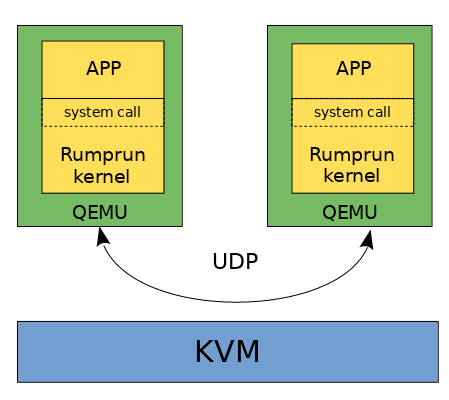
\includegraphics[scale=0.7]{figures/pipe_stage2.png}
%%\caption{Δεύτερο στάδιο υλοποίησης μηχανισμού pipe\label{fig4_3}}
%%\end{figure}
%%------------------------------------------------------------------------------
%%------------------------------------------------------------------------------

\subsubsection{Στάδιο 3 - pipe ως function call με shared memory}

Στο τελευταίο στάδιο, υλοποιήσαμε το μηχανισμό pipe, πάλι ως system call με τη
διαφορά ότι πλέον δε χρησιμοποιούνται sockets, αλλά κοινή μνήμη μεταξύ των
εικονικών μηχανημάτων. Πλέον δεν υπάρχει ανάγκη για ύπαρξη δικτύου μεταξύ των
εικονικών μηχανημάτων, ωστόσο η συγκεκιμένη υλοποίηση μπορεί να χρησιμοποιηθεί
μόνο για unikernels, που μοιράζονται τον ίδιο host. Για την κοινή μνήμη
χρησιμοποιήθηκε το ivshmem \cite{macdonell2011shared}. Όπως έχει ήδη αναφερθεί
πρόκειται για ένα μηχανισμό, που επιτρέεπει το διαμοιρασμό μνήμης μεταξύ του
host και των εικονικών μηχανών που εκτελούνται στο host. Η χρήση του γίνεται
μέσω μίας PCI συσκευής. Συνεπώς έπρεπε να δημιουργήσουμε τον κατάλληλο driver
που θα μας επιστρέψει να το χρησιμοποιήσουμε. Στην παρακάτω εικόνα \ref{fig4_4}
φαίνεται σχηματικά η υλοποίηση. 

\begin{figure}[htp]
\centering
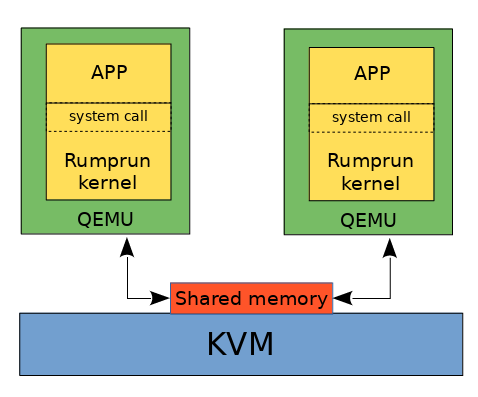
\includegraphics[scale=0.7]{figures/pipe_stage3.png}
\caption{Τρίτο στάδιο υλοποίησης μηχανισμού pipe\label{fig4_4}}
\end{figure}

Η χρήση του pipe, από την εφαρμογή γίνεται πλέον όπως σε κάθε UNIX λειτουργικό
σύστημα. Καλώντας την pipe, αν όλα πάνε καλά αποθηκεύονται στις
παραμέτρους fildes[0], fildes[1], οι δύο file descriptors που θα χρησιμοποιηθούν
για την ανάγνωση και εγγραφή αντίστοιχα. Σε περίπτωση επιτυχίας επιστρέφεται η
τιμή 0, ενώ σε αντίθετη περίπτωση, στη μεταβλητή errno αποθηκεύεται ο κωδικός
του σφάλματος. Επιπλέον έχουν υλοποιηθεί και όσα semantics δεν είχαν υλοποιηθεί
στα προηγούμενα στάδια. Οπότε, σε περίπτωση που δεν υπάρχουν ανοιχτά άκρα
ανάγνωσης στο pipe, η εγγραφή δε θα είναι επιτυχής. Αν δεν υπάρχει αρκετός χώρος
για την εγγραφή δεδομένων, τότε η write "μπλοκάρει".

Θα ξεκινήσουμε την περιγραφή της υλοποίησης από την υλοποίηση του PCI driver για
το ivshmem. Αρχικά πρέπει να ενημερώσουμε το qemu για τη χρήση του συγκεκριμένου
μηχανισμού. Για να γίνει αυτό χρησιμοποιούμε τις ακόλουθες παραμέτρους για το qemu.
\begin{lstlisting}[numbers=none]
-device ivshmem-plain,memdev=hostmem -object memory-backend-file,size=1M,share,mem-path=/dev/shm/ivshmem,id=hostmem
\end{lstlisting}
%% TODO na dw an isxuei auto pou grafw me to mempath
Στην παράμετρο size, ορίζουμε τη χωρητικότητα του pipe και για κάθε pipe πρέπει
να ορίσουμε διαφορετικό mem-path. Κάθε unikernel που ξεκινάει με τις
συγκεκριμένες παραμέτρους μπορεί να χρησιμοποιήσει το pipe. 

Από τη μεριά του unikernel, χρειάζεται να κατασκευάσουμε έναν PCI driver για το
μηχανισμό ivshmem. Όπως και στην περίπτωση του system call έτσι και στην
περίπτωση του driver, αρχικά πρέπει να φτιάξουμε το driver για το NetBSD. 
Ακολουθώντας το Kernel Development Manual του NetBSD ~\cite{NetBSDKDMDriver},
για τον pci device driver υλοποιήσαμε τρεις συναρτήσεις:
\begin{enumerate}
	\item match: Είναι η συνάρτηση που καλείται από το autoconfiguration
		framework του NetBSD, όταν το σύστημα εκκινεί, ώστε να
		ταιριαστεί ο driver με τη συσκευή. Οπότε στην περίπτωση του
		δικού μας driver η συγκεκιμένη συνάρτηση ελέγχει αν πρόκειται
		για ivshmem pci device, ελέγχοντας τις τιμές του κατασκευαστή
		και το id της συσκευής.
	\item attach: Καλείται μόνο αν η ανίσχνευση της συσκευής ήταν επιτυχής
		(αν η match επέστρεψε 1). Ο ρόλος της είναι να αρχιοποιήσει τη
		συκευή. Δεδομένου, ότι εμείς χρησιμοποιούμε το συγκεκριμένο
		μηχανισμό απλά για διαμοιρασμό μνήμης, αρκεί να κάνουμε map το
		PCI\_BAR(2) του ivshmem και να αποθηκεύσουμε τις απαραίτητες
		μεταβλητές για τη χρήση του μηχανισμού.
	\item detach: Καλείται σε περίπτωση που η συσκευή αποσυνδεθεί. Στη δική
		μας περίπτωση είναι αρκετό να κάνουμε unmap το bus\_space που
		χρησιμοποιούμε και να μηδενίσουμε τις μεταβλητές που
		χρησιμοποιούμε για τη συσκευή.
\end{enumerate}

Προκειμένου να μπορεί να χρησιμοποιηθεί η συσκευή από τον υπόλοιπο πυρήνα του
NetBSD, είναι απαραίτητο να αποθηκευτούν οι απαραίτητες μεταβλητές που
αναφέρθηκαν στις συναρτήσεις attach και detach. Για το λόγο αυτό δημιουργήθηκε
το struct ivshm, που έχει ως πεδία τις μεταβλητές αυτές. 
\begin{lstlisting}[numbers=none]
struct ivshm {
	bus_size_t		data_s;	/* size of shared memory */
	bus_addr_t		data_b;	/* base address of shared memory */
	bus_space_tag_t		data_t;	/* bus tag for shared memory */
	bus_space_handle_t	data_h;	/* bus handle for shared memory */
};
\end{lstlisting}
Ιδανικά θα θέλαμε να κάνουμε map όλη την κοινή μνήμη του ivshmem, ώστε να μπορεί
να χρησιμοποιηθεί σαν μνήμη του πυρήνα. Ωστόσο, το rumprun δεν υποστηρίζει το
maping μνήμης μέσω του bus. Ως εκ τούτου, η πρόσβαση στην κοινή μνήμη γίνεται
κάθε φορά με εγγραφή και ανάγνωση bytes από αυτήν χρησιμοποιώντας το bus. Υπό
αυτές τις συνθήκες, υπήρχαν τέσσερις μεταβλητές που ήταν απαραίτητες:
\begin{enumerate}
	\item το μέγεθος της κοινής μνήμης.
	\item η διεύθυνση βάσης της κοινής μνήμης
	\item το bus tag της κοινής μνήμης
	\item και το bus handle της κοινής μνήμης.
\end{enumerate}
Οι 2 τελευταίες μεταβλητές, είναι αυτές που χρησιμοποιούνται από τις συναρτήσεις
που παρέχει το NetBSD για να μπορέσει χρησιμοποιώντας το bus, να επικοινωνήσει
με τη συσκευή. Ο ρόλος των υπόλοιπων δύο μεταβλητών θα γίνει πιο ξεκάθαρος
παρακάτω.

Αφού λοιπόν, δημιουργήσαμε το driver για το NetBSD και ενημερώσαμε το
autoconfiguration framework για την ύπαρξη του, έπρεπε να κάνουμε γνωστή την
ύπαρξη του και στο rumprun. Για να γίνει αυτό απαιτούνται δύο ενέργεις. Πρώτον
προσθέτουμε το pci driver στο src-netbsd/sys/rump/dev/Makefile.rumpdevcomp.
Δεύτερον, να δημιουργηθεί ένα νέο directory στο src-netbsd/sys/rump/dev/lib/ για
τη νέα συσκευή. Το directory υατό περιέχει το ioconf και το απαραίτητο Makefile
για να προστεθεί o οδηγός μας στο build σύστημα του rumprun. 

\begin{lstlisting}[caption={IVSHMEM.ioconf},captionpos=b]
ioconf ivshmem

include "conf/files"
include "dev/pci/files.pci"
include "rump/dev/files.rump"

pseudo-root pci*

ivshmem* at pci? dev ? function ?
\end{lstlisting}

\begin{lstlisting}[caption={rumprun Makefile για το ivshmem},captionpos=b]
RUMPTOP=${TOPRUMP}

.PATH:	${RUMPTOP}/../dev/pci

LIB=	rumpdev_ivshmem
COMMENT=ivshmem

IOCONF=	IVSHMEM.ioconf
RUMP_COMPONENT=ioconf

SRCS+=	ivshmem.c
##SRCS+=	ivshmem_component.c

CPPFLAGS+= -I${RUMPTOP}/librump/rumpkern

.include "${RUMPTOP}/Makefile.rump"
.include <bsd.lib.mk>
.include <bsd.klinks.mk>
\end{lstlisting}

Η αρθρωτή οργάνωση των unikernels, δίνει τη δυνατότητα κάθε φορά να επιλέγονται
μόνο τα απαραίτητα συστατικά για κάθε unikernel. Σε αυτό αποσκοπεί και η
δημιουργία του παραπάνω directory, ώστε να μπορεί ο συγκεκιμένος driver να
ενσωματωθεί στο unikernel, κατά τη διάρκεια του baking. Για τη χρήση του
συγκεκριμένου οδηγού είναι απαραίτητη η εισαγωγή του -lrumpdev\_ivshmem στο
config με το οποίο θα γίνει bake η εφαρμογή. 

Αφού δημιουργήσαμε τον driver, το επόμενο βήμα ήταν η αλλαγή του system call,
ώστε αντί για sockets να χρησιμοποιείται ο μηχανισμός του ivshmem. Αρχικά, δε
χρειαζόμαστε την ioctl κλήση και δημιουργούμε δύο structs, το struct pipe και το
struct pipe\_op. Οι ορισμοί τους φαίνονται παρακάτω:

\begin{lstlisting}
struct pipe {
	bus_size_t	init;		/* is shared memory initalized? */
	bus_size_t	lock;		/* pipe lock */
	bus_size_t	wr_lock;	/* writers lock */
	bus_size_t	nreaders;	/* number of readers in pipe */
	bus_size_t	nwriters;	/* number of writers in pipe */
	bus_size_t	len;		/* size of pipe buffer */
	bus_size_t	in;		/* pointer for next write */
	bus_size_t	out;		/* pointer for next read */
	bus_size_t	cnt;		/* number of bytes in pipe */
	bus_size_t	buf;		/* pipe buffer */
	int		pr_readers;	/* readers from this process */
	int		pr_writers;	/* writers from curr process */
};

struct pipe_op {
	int		oper;		/* operation in pipe 0 for read,
					   1 for write*/
	struct pipe	*pipe;
};
\end{lstlisting}

Το struct pipe\_op συνδέεται με τα file descriptors που δημιουργεί η κλήση pipe,
ένα για κάθε file descriptor. H μεταβλητή oper, καθορίζει αν πρόκειται για το
file descriptor που αφορά την εγγραφή στο pipe ή αυτό που αφορά στην ανάγνωση. η
άλλη τιμή είναι το struct pipe που είναι κοινό και για τα δύο άκρα του pipe και
περιέχει βοηθητικές μεταβλητές για τη διαχείρηση του pipe. Όπως έχει ήδη
αναφερθεί η χρήση της κοινής μνήμης γίνεται μέσω του bus και οι συναρτήσεις
εγγραφής ή ανάγνωσης από το bus απαιτούν ως παράμετρο τη διεύθυνση βάσης από την
οποία θα διαβαστούν τα δεδομένα. Έτσι για να αναφερθούμε σε διαφορετική
μεταβλητή μέσα σε αυτή τη μνήμη θα πρέπει να χρησιμοποιήσουμε διαφορετική
διεύθυνση βάσης. Συνεπώς, το struct pipe περιέχει τις διευθύνσεις των κοινών
μεταβλητών στην κοινή μνήμη. Επιπλέον, χρησιμοποιούνται και οι μεταβλητές
pr\_readers και pr\_writers που αφορούν τα ανοιχτά άκρα στο pipe από τη
συγκεκριμένη διεργασία. Η δύο τελευταίες μεταβλητές είναι απαραίτητες για τη
διαχείρηση του pipe όταν η διεργασία που έχει δημιουργήσει το pipe κάνει fork.

\begin{figure}[htp]
\centering
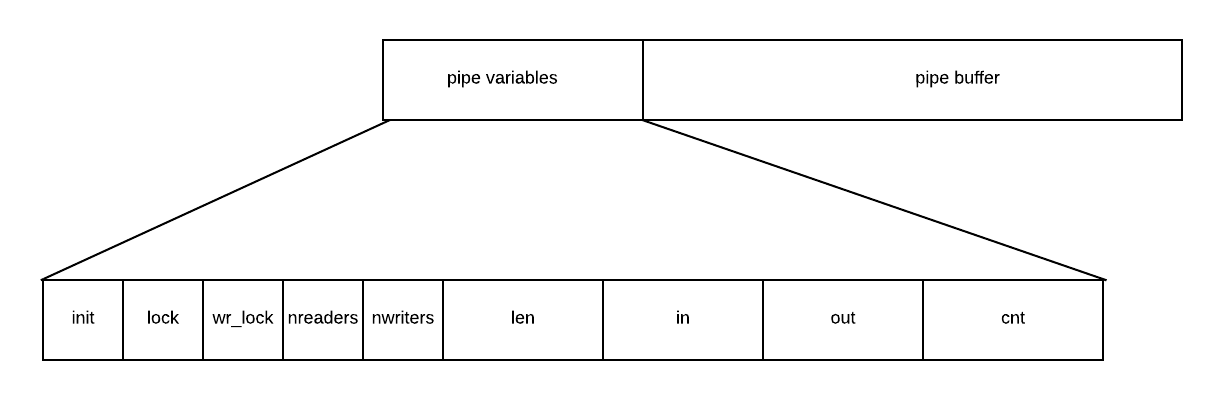
\includegraphics[scale=0.7]{figures/shared_memoery_layout.png}
\caption{shared memory layout\label{fig4_5}}
\end{figure}

Αν θεωρήσουμε την κοινή μνήμη σαν ένα μεγάλο συνεχόμενο κομμάτι μνήμης, τότε
στην παραπάνω εικόνα ~\ref{fig4_5} φαίνεται πως την έχουμε διαχωρίσει εσωτερικά,
με ένα κομμάτι της να αφορά τις μοιραζόμενες μεταβλητές και ένα άλλο τον buffer
του pipe. Οι αρχικές μεταβλητές, έχουν μικρότερο μέγεθος από τις τελευταίες και
η λειτουργία της κάθε μίας έχει ώς εξής:
\begin{itemize}
	\item init: Πρόκειται για μία μεταβλητή ελέγχου, που καθορίζει αν έχουν
		αρχικοποιηθεί οι κοινές μεταβλητές του pipe. Αλλάζεις μόνο δύο
		φορές, όταν πρωτοδημιουργείται το pipe και όταν αυτό
		καταστρέφεται. Ουσιαστικά δηλώνει αν οι υπόλοιπες μεταβλητές
		περιέχουν "σκουπίδια", ή αν έχουν χρήσιμες τιμές.
	\item lock: Πρόκειται για το γενικό lock του pipe και προστατεύει όλες
		τις κοινές μεταβλητές του pipe. 
	\item wr\_lock: Πρόκειται για ένα lock που κάθε φορά επιτρέπει σε ένα
		και μόνο unikernel ννα γράφει στο pipe. 
	\item nreaders: Ο αριθμός των ανοιχτών άκρων ανάγνωσης για το pipe
	\item wreaders: Ο αριθμός των ανοιχτών άκρων εγγραφής για το pipe
	\item len: Το μέγεθος του pipe buffer.
	\item in: Ο δείκτης που καθορίζει σε ποιο σημείο θα γραφτούν τα νέα
		δεδομένα στο pipe buffer.
	\item out: Ο δείτης που καθορίζει από ποιο σημείο θα διβαστούν δεδομένα
		από το pipe buffer
	\item cnt: Μετρητής των bytes που υπάρχουν στο pipe, κάθε στιγμή
\end{itemize}

Για την πρόσβαση στις παραπάνω μεταβλητές και γενικά για την κοινή μνήμη
χρησιμοποιήθηκαν οι συναρτήσεις bus\_space\_read\_1, bus\_space\_read\_4,
bus\_space\_write\_1, bus\_space\_write\_4. Ο αριθμός στο τέλος της κάθε
συνάρτησης υποδηλώνει το μέγεθος των δεδομένων που θα διαβαστούν ή θα γραφτούν.
Για την πιο εύκολη χρήση της κοινής μνήμης δημιουργήθηκαν 4 βοηθητικές
συναρτήσεις, που φαίνονται παρακάτω. 

\begin{lstlisting}
/*
 * Read a region of bytes in bus (data is 1 byte)
 */
void read_region_1(bus_size_t offset, uint8_t *datap, bus_size_t count)
{
	int i;
	for (i=0; i<count; i++) {
		datap[i] = bus_space_read_1(sharme.data_t, sharme.data_h,
				offset + i);
	}
	return;
}

/*
 * Read a region of bytes in bus (data is 4 byte)
 */
void read_region_4(bus_size_t offset, uint32_t *datap, bus_size_t count)
{
	int i;
	for (i=0; i<count; i++) {
		datap[i] = bus_space_read_4(sharme.data_t, sharme.data_h,
				offset + i*4);
	}
	return;
}

/*
 * Write in a region of bytes in bus (data is 1 byte)
 */
void write_region_1(bus_size_t offset, uint8_t *datap, bus_size_t count)
{
	int i;
	for (i=0; i<count; i++) {
		bus_space_write_1(sharme.data_t, sharme.data_h, offset + i,
				datap[i]);
	}
	return;
}

/*
 * Write in a region of bytes in bus (data is 4 byte)
 */
void write_region_4(bus_size_t offset, uint32_t *datap, bus_size_t count)
{
	int i;
	for (i=0; i<count; i++) {
		bus_space_write_4(sharme.data_t, sharme.data_h,	offset + i*4,
				datap[i]);
	}
	return;
}
\end{lstlisting}

Οι παραπάνω συναρτήσεις διαβάζουν ή γράφουν σε μία περιοχή μνήμης, είτε 1 είτε 4
bytes δεδομένα. Το μέγεθος της περιοχής που θα γίνει η πρόσβαση καθορίζεται από
την παράμετρο count και το μέγεθος των bytes (count * bytes\_of\_data). Οι άλλες
2 παράμετροι των συναρτήσεων είναι η διεύθυνση βάσης για το bus και ένας πίνακας
, στον οποίο αποθηκεύονται τα δεδομένα που διαβάστηκαν από μνήμη είτε τα
δεδομένα που θα γραφτούν στην περίπτωση, στις λειτουργίες read και write
αντίστοιχα. Οι συναρτήσεις bus\_space, χρησιμοποιούν τη δομή struct ivshm, για
τις μεταβλητές bus tag και bus handle. Όλες οι αναφορές στην κοινή μνήμη, πέρα
από αυτές των locks, γίνονται χρησιμοποιώντας αυτές τις συναρτήσεις.

Η ύπαρξη κοινής μνήμης μεταξύ διαφορετικών unikernels, απαιτεί και την ύπαρξη
κάποιου συγχρονισμού μεταξύ αυτών. Για αυτό σκοπό χρησιμοποιούνται τα δύο locks
στο struct pipe (lock, wr\_lock). Τα δύο αυτά locks, βρίσκονται εντός της κοινής
μνήμης και απαιτούν ειδική μεταχείριση. Ο μηχανισμός ivshmem μπορεί να
υποστηρίξει τη χρήση ατομικών εντολών του gcc. Για το λόγο, αυτό δημιουργήσαμε
δύο ακόμα συναρτήσεις για το locking, μία για την απόκτηση του κλειδώματος και
μία για την απελευθέρωση του. Ου συναρτήσεις αυτές φαίνονται παρακάτω. 

\begin{lstlisting}
/*
 * Spinlock for pipe
 */
void pipe_lock(bus_size_t lock)
{
	while(__sync_val_compare_and_swap((uint8_t *)sharme.data_b + lock, 0, 1) == 1)
		/* do nothing */;
	return;
}

/*
 * Release the lock
 */
void pipe_unlock(bus_size_t lock)
{
	__sync_lock_release((uint8_t *)sharme.data_b + lock);
	return;
}

\end{lstlisting}

Οι ατομικές εντολές που χρησιμοποιήθηκαν για τη χρήση του lock, είναι οι
\_\_sync\_val\_compare\_and\_swap και \_\_sync\_lock\_release. Οι εντολές αυτές
δέχονται ως παράμετρο τη διεύθυνση της μνήμης στην οποία θα γίνει η πρόσβαση. Η
διεύθυνση αυτή καθορίζεται από τη διεύθυνση βασης των δεδομένων (data\_b) στο
struct ivshmem και το offset του lock μέσα στην κοινή μνήη που είναι
αποθηκευμένο στο struct pipe. Οποιαδήποτε αλλαγή σε κάποιο κομμάτι της κοινή
μνήμης απαιτεί την απόκτηση του γενικού lock, ενώ οποιαδήποτε εγγραφή στο pipe
θα πρέπει να έχει πάρει τον έλεγχο του wr\_lock.

Όταν λοιπόν, η εφαρμογή που εκτελείται σε ένα unikernel εκτελέσει την κλήση
pipe, από τη μεριά του πυρήνα πέρα από τη δημιουργία των file descriptors και τη
σύνσεση τους με το εκάστοτε struct pipe\_op συμβαίνουν τα εξής. Αρχικά,
δημιουργείται το struct pipe και αρχικοποιούνται όλες οι μεταβλητές τους με το
offset της κάθε μίας στην κοινή μνήμη. Ύστερα, ξεκινά ο έλεγχος της κοινής
μνήμης. Ελέγχεται η τιμή της init στην κοινή μνήμη και ανάλογα με την τιμή της η
κοινή μνήμη, είτε θα αρχικοποιειθεί είτε όχι. Στη συνέχεια, αφού η περιοχή
μνήμης έχει αρχικοποιηθεί, αυξάνονται οι μετρητές των άκρων του pipe και τέλος
συνδέεται το κοινό struct pipe με τα struct pipe\_op. Η κλήση επιστρέφει τους
file descriptors στην εφαρμογής και το pipe είναι πλέον έτοιμο να
χρησιμοποιηθεί. Ειδική σημείωση πρέπει να γίνει για τον έλεγχο της τιμής init
στην κοινή μνήμη. Η κοινή μνήμη πρέπει να καταστραφεί, αν δεν υπάρχουν pipes που
τη χρησιμοποιούν καθώς σε διαφορετική περίπτωση μπορεί λόγω του τρόπου ελέγχου
της init, να μην αρχικοποιηθεί. 

Σημαντικό ρόλο στον παραπάνω σκοπό έχει η κλήση close σε ένα file descriptor του
pipe. Στην απλή περίπτωση που δεν πρόκειται για το τελευταίο file descriptor του
pipe, απλά ενημερωονται οι μετρητές των ανοιχτών άκρων του pipe. Αν όμως,
πρόκειται να κλείσει το τελευταίο file descriptor που αφορά το συγκεκριμένο pipe
τότε μηδενίζεται όλη η κοινή μνήμη που χρησιμοποιήθηκε. Με αυτό τον τρόπο την
επόμενη φορά που θα χρησιμοποιηθεί το συγκεκριμένο κομμάτι μνήμης η τιμή init θα
υποδηλώνει ότι πρέπει η κοινή μνήμη να αρχικοποιηθεί. 

\begin{figure}[htp]
\centering
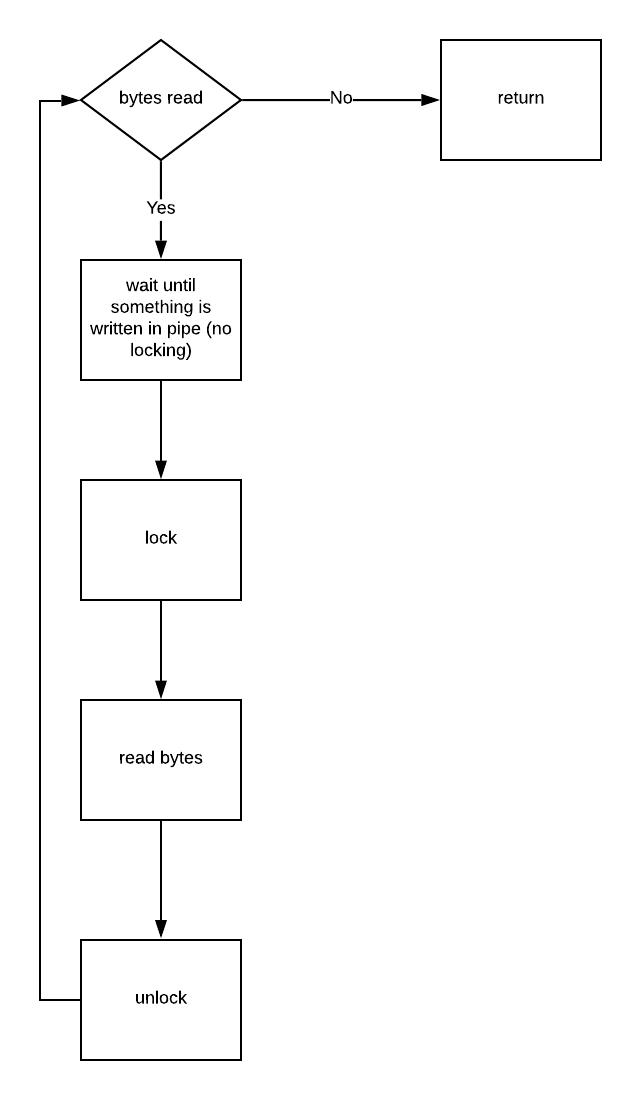
\includegraphics[scale=0.7]{figures/pipe_read.png}
\caption{pipe read flow chart\label{fig4_6}}
\end{figure}

Στην παραπάνω εικόνα ~\ref{fig4_6} φαίνεται το διάγραμμα ροής, όταν εκτελείται η
κλήση read σε άκρο ανάγνωσης του pipe. Ουσιαστικά πρόκειται για ένα while loop,
το οποίο τερματίζει υπό τέσσερις ορισμένες συνθήκες:
\begin{enumerate}
	\item Αν έχουν διαβαστεί όσα bytes ζήτησε η εφαρμογή
	\item Αν έχουν διαβαστεί όλα τα bytes από το pipe (ανεξάρτητα από τα
		πόσα ζήτησε η εφαρμογή) 
	\item Αν δεν υπάρχουν δεδομένα να διαβαστούν και όλα τα άκρα εγγραφής
		έχουν κλείσει
	\item Αν κάτι πάει στραβά κατά τη διαδικασία μεταφοράς δεδομένων από την
		κοινή μνήμη στην εφαρμογή.
\end{enumerate}
Για την αποφυγή deadlocks, αρχικά γίνεται έλεγχος για τη διαθεσιμότητα δεδομένων
στο pipe χωρίς την απόκτηση του γενικού κλειδώματος. Σε περίπτωση, που υπάρχουν
δεδομένα, τότε αποκτάται το κλείδωμα και επαναλαμβάνεται ο έλεγχος με την κατοχή
του κλειδώματος. Αφού λοιπόν μεταφερθύν τα δεδομένα από την κοινή μνήμη στην
εφαρμογή, τότε ενημερώνονται οι κοινές μεταβλητές του pipe (out, cnt) και
ελευθερώνεται το lock. Καθώς ο buffer του pipe είναι κυκλικός, πρέπει να
λαμβάνουμε υπόψιν την περίπτωση που έχουμε φτάσει στο τέλος του buffer, οπότε
πρέπει να ξεκινήσουμε να διαβάζουμε τα υπόλοιπα δεδομένα από την αρχή. Τέλος,
τόσο κατά τη διάρκεια του ελέγχου δεδομένων χωρίς αλλά και με το κλείδωμα,
ελέγχονται και τα ανοιχτά άκρα εγγραφής στο pipe. Αν όλα έχουν κλείσει τότε
πρέπει να επιστρέψει η κλήση pipe καθώς δεν πρόκειται να εγγραφούν νέα δεδομένα.

\begin{figure}[htp]
\centering
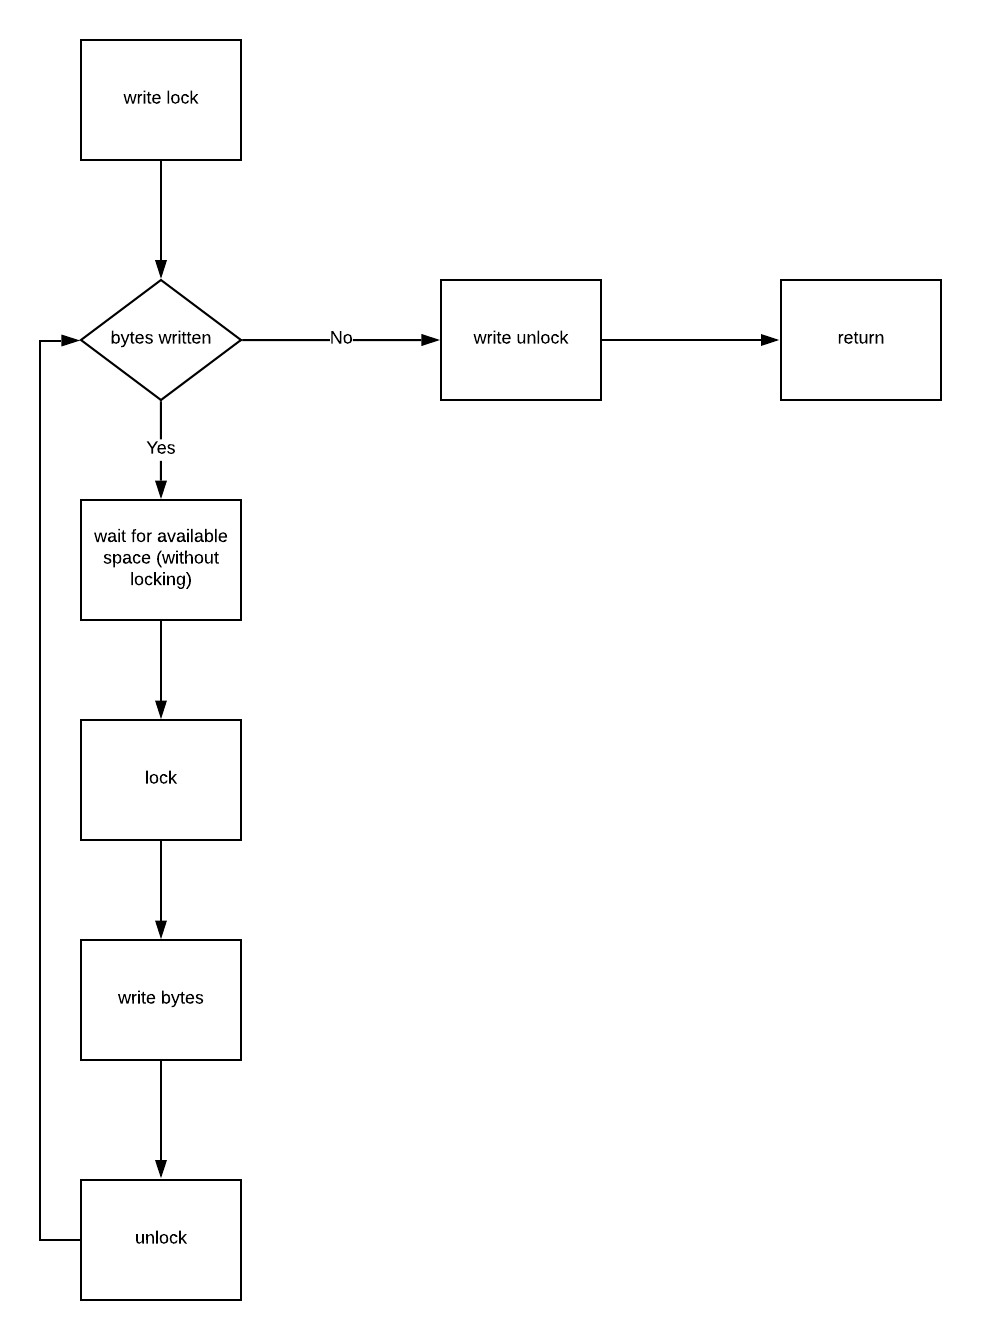
\includegraphics[scale=0.7]{figures/pipe_write.png}
\caption{pipe write flow chart\label{fig4_7}}
\end{figure}

Στην παραπάνω εικόνα ~\ref{fig4_7} φαίνεται το διάγραμμα ροής της κλήσης write
του pipe. Όπως φαίνεται δεν έχει κάποια ιδιαίτερη διαφορά με το διάγραμμα ροής
της κλήσης read, εκτός από το γεγονός ότι από την αρχή μέχρι το τέλος της
εκτέλεσης της δεσμεύεται το wr\_lock. Ο λόγος ύπαρξης ενός τέτοιου κλειδώματος,
είναι για να επιτευχθεί η ατομικότητα της κλήσης write σε ένα pipe. Από εκεί και
πέρα, όπως και πριν αρχικά ελέγχουμε αν υπάρχει διαθέσιμος χώρος στην κοινή
μνήμη για την εισαγωγή νέων δεδομένων. Έπειτα αποκτάται το κλείδωμα και
επαναλαμβάνεται ο έλεγχος διαθέσιμου χώρου. Αν είναι επιτυχής, γίνεται η εγγραφή
δεδομένων στην κοινή μνήμη και ενημερώνονται οι αντίστοιχες μεταβλητές (in,
cnt). Καθώς οbuffer του pipe είναι κυκλικός πρέπει να λαμβάνουμε υπόψιν την
περίπτωση που ο διαθέσιμος χώρος βρίσκεται την αρχή του buffer. Τόσο κατά τη
διαδικασία ελέγχου διαθέσιμου χώρου χωρίσς κλείδωμα όσο και με κλείδωμα,
ελέγχονται και τα ανοιχτά άκρας ανάγνωσης του pipe. Αν όλα έχουν κλείσει τότε
πρέπει να επιστρέψει η κλήση pipe με το error EPIPE, καθώς δεν υπάρχουν
αναγνώστες να διαβάσουν τα δεδομένα. Τέλος, ´ολα τα παραπάνω βρίσκονται μέσα σε
ένα while loop το οποίο μπορεί να τερματίσει υπό τις τέσσερις παρακάτω συνθήκες.
\begin{enumerate}
	\item Αν έχουν γραφτεί όσα bytes ζήτησε η εφαρμογή
	\item Αν δεν υπάρχει κανένα ανοιχτό άκρο ανάγνωσης στο pipe.
	\item Αν κάτι πάει στραβά κατά τη διαδικασία μεταφοράς δεδομένων από την
		την εφαρμογή στην κοινή μνήμη.
\end{enumerate}

\subsection{Στάδια υλοποίησης}


